Исходными данными для модели являются: информация о составе файлов исходного кода, сведения об их зависимостях между друг другом, а так же трассируемость требований на них.

Перед началом работы модели необходимо определить:
\begin{enumerate}
    \item множество файлов исходного кода $F_{sc}^* = \{F_{sc}^1, F_{sc}^2, ..., F_{sc}^{n}\}$;
    \item множество требований к ПО $R^* = \{R^1, R^2, ..., R^m\}$.
    \item матрицу бинарных отношений трассируемости требований к ПО на файлы исходного кода $Mt$ размерности $n \times m$;
    \item матрицу бинарных отношений зависимостей файлов исходного кода $Md$ размерности $n \times n$.
\end{enumerate}

Значение элемента $a_{i,j}^{Mt}$ матрицы $Mt$ определяется следующим образом:

$
a_{i,j}^{Mt} = \begin{cases}
    1  & \quad \text{если файл } F_{sc}^i \text{ реализует требование } R^j\\
    0  & \quad \text{если файл } F_{sc}^i \text{ не реализует требование } R^j
  \end{cases}
$

Значение элемента $a_{i,j}^{Md}$ матрицы $Md$ определяется следующим образом:

$
a_{i,j}^{Md} = \begin{cases}
    1  & \quad \text{если файл } F_{sc}^i \text{ имеет зависимость на файл } F_{sc}^j\\
    0  & \quad \text{если файл } F_{sc}^i \text{ не имеет зависимость на файл } F_{sc}^j \text{ или } i = j\\
  \end{cases}
$

Примеры исходных матриц $Mt$ и $Md$ приведены в таблицах \ref{tab:requirements_traceability_matrix} и \ref{tab:dependency_matrix} соответственно.

\begin{longtable}{|c|c|c|c|c|}
\caption{Пример матрицы трассируемости требований на файлы исходного кода}
\label{tab:requirements_traceability_matrix}\\
\hline
& \cellcolor{ash-grey} $R^1$ 
& \cellcolor{ash-grey} $R^2$ 
& ... 
& \cellcolor{ash-grey} $R^m$ \\
\hline
\cellcolor{platinum} $F_{sc}^1$ & \cellcolor{light-colar} 1 & 0 & ... & 0 \\
\hline
\cellcolor{platinum} $F_{sc}^2$ & 0 & \cellcolor{light-orange} 1 & ... & 0 \\
\hline
\cellcolor{platinum} $F_{sc}^3$ & 0 & \cellcolor{crayola} 1 & ... & 0 \\
\hline
... & ... & ... & ... & ... \\
\hline
\cellcolor{platinum} $F_{sc}^n$ & 0 & 0 & ... & \cellcolor{light-green} 1 \\
\hline
\end{longtable}

\begin{longtable}{|c|c|c|c|c|c|}
\caption{Пример матрицы зависимостей между файлами исходного кода}
\label{tab:dependency_matrix}\\
\hline
& \cellcolor{platinum} $F_{sc}^1$ 
& \cellcolor{platinum} $F_{sc}^2$ 
& \cellcolor{platinum} $F_{sc}^3$ 
& ... 
& \cellcolor{platinum} $F_{sc}^n$ \\
\hline
\cellcolor{platinum} $F_{sc}^1$ & 0 & 0 & \cellcolor{light-blue} 1 & ... & 0 \\
\hline
\cellcolor{platinum} $F_{sc}^2$ & 0 & 0 & 0 & ... & 0 \\
\hline
\cellcolor{platinum} $F_{sc}^3$ & \cellcolor{mauve} 1 & 0 & 0 & ... & 0 \\
\hline
... & ... & ... & ... & ... & ... \\
\hline
\cellcolor{platinum} $F_{sc}^n $ & 0 & 0 & 0 & ... & 0 \\
\hline
\end{longtable}

По входным данным строится изначальный граф $G$. В $G$ выделяются два слоя:
\begin{enumerate}
    \item слой файлов исходного кода;
    \item слой требований к ПО.
\end{enumerate}

Пример $G$, построенного по входным данным, приведен на рисунке~\ref{fig:original_count}.

\begin{figure}[H]
    \centering
    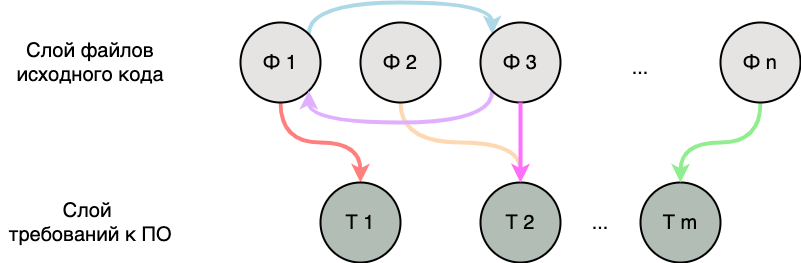
\includegraphics[width=1\textwidth]{original_count}
    \caption{Пример изначального графа}
    \label{fig:original_count}
\end{figure}

% Требование на модель
Разрешение циклических зависимостей графовой математической модели трассируемости требований к ПО на файлы исходного кода происходит в несколько этапов:
\begin{enumerate}
    \item считывание $F_{sc}^*$, $R^*$, $Mt$ и $Md$;
    \item построение $G$ аналогично подходу, описанному в [8];
    \item выполнятся коррекция аналогично описанным в~[9, 14] подходам пока в $G$ на слое файлов исходного кода присутствуют циклы. В работе описываемой модели выполняется слияние~[7] входящих в цикл вершин:
    \begin{itemize}
        \item дуги между сливающимися вершинами удаляются;
        \item образованная группа является новой вершиной графа, при этом все входящие и исходящие дуги замыкаются на нее. Пример слияния приведен на рисунке~\ref{fig:merge_example};
    \end{itemize}
    \item формирование результирующего графа трассируемости $G'$.
\end{enumerate}

\begin{figure}[H]
    \centering
    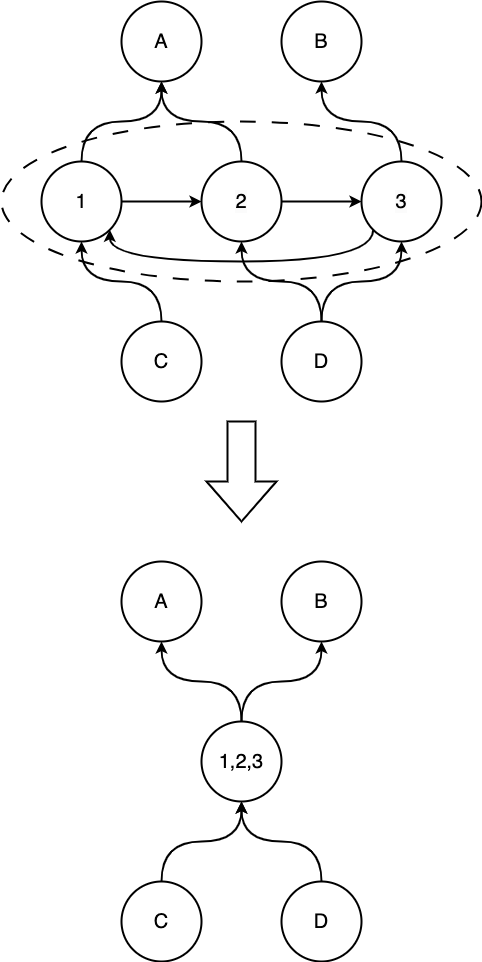
\includegraphics[width=0.5\textwidth]{merge_example}
    \caption{Пример слияния входящих в цикл вершин}
    \label{fig:merge_example}
\end{figure}

На следующей итерации поиска циклов в графе вышеобозначенные группы учитываются как обычные вершины и таким образом могут участвовать в образовании новых групп по вышеуказанным правилам.

В приведенном примере (см рис.~\ref{fig:original_count}) вершины $F_{sc}^1$ и $F_{sc}^3$ образуют цикл. Результат слияния приведен на рисунке \ref{fig:result_count}.

\begin{figure}[H]
    \centering
    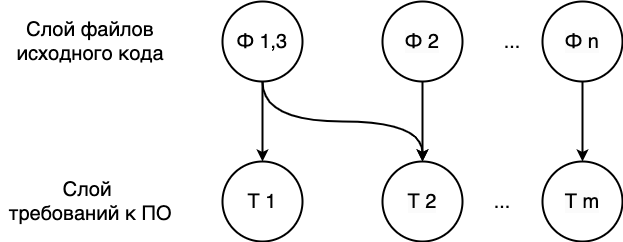
\includegraphics[width=0.8\textwidth]{result_count}
    \caption{Пример результирующего графа}
    \label{fig:result_count}
\end{figure}

Результирующий граф может быть использован при оценке объема верификационных процедур, которые необходимо выполнить при внесении изменений в файлы исходного кода. Так, при внесении изменений в файл исходного кода $F_{sc}^1$ требуется выполнить верификационные процедуры реализации требований $R^1$ и $R^2$.